\documentclass[a4paper]{article}
\usepackage[utf8]{inputenc}
\usepackage[spanish, es-tabla, es-noshorthands]{babel}
\usepackage[table,xcdraw]{xcolor}
\usepackage[a4paper, footnotesep = 1cm, width=18cm, left=2cm, top=2.5cm, height=25cm, textwidth=18cm, textheight=25cm]{geometry}
%\geometry{showframe}

\usepackage{amsmath}
\usepackage{amsfonts}
\usepackage{amssymb}
\usepackage{float}
\usepackage{graphicx}
\usepackage{caption}
\usepackage{subcaption}
\usepackage{multicol}
\usepackage{multirow}
\setlength{\doublerulesep}{\arrayrulewidth}

\graphicspath{{../Ejercicio-1/}{../Ejercicio-2/}{../Ejercicio-3y4/}{../Ejercicio-5-6y7/}{../Ejercicio-8/}}

\usepackage{hyperref}
\hypersetup{
    colorlinks=true,
    linkcolor=blue,
    filecolor=magenta,      
    urlcolor=blue,
    citecolor=blue,    
}
\newcommand\underrel[2]{\mathrel{\mathop{#2}\limits_{#1}}}
\newcommand{\quotes}[1]{``#1''}
\usepackage{array}
\newcolumntype{C}[1]{>{\centering\let\newline\\\arraybackslash\hspace{0pt}}m{#1}}
\usepackage[american,oldvoltagedirection,siunitx]{circuitikz}
\usepackage{fancyhdr}
\usepackage{units}
\usepackage{booktabs}

\usepackage{tikz}
\usetikzlibrary{babel}

\pagestyle{fancy}
\fancyhf{}
\lhead{22.42 Laboratorio de Electrónica}
\rhead{Bertachini, Lambertucci, Londero Bonaparte, Mechoulam, Scapolla}
\rfoot{\center \thepage}

\begin{document}
	\section{Introducción}

El presente trabajo de laboratorio tiene como objetivo estudiar distintos tipos de puentes. En la primera sección se presenta el concepto de equilibrio de puentes y se analizan distintos métodos para medir cuándo un puente ha llegado al equilibrio. En la segunda parte se estudia y diseña un puente de Wien, capaz de medir frecuencias. En la tercera parte se diseña un puente para medir capacitores. 

\section{Métodos de medición de quilibrio de puentes}
\begin{figure}[H]
	\centering
	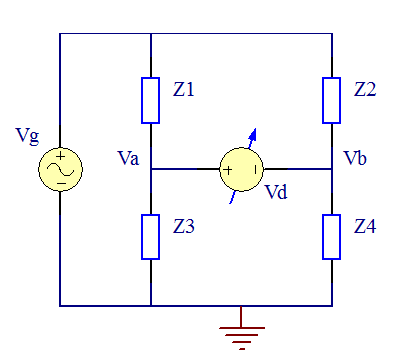
\includegraphics[width=0.4\textwidth]{/ImagenesEjercicio1/puente.png}
\caption{Puente}
	\label{fig:pte}
\end{figure}


Considérese el puente de la figura 1. Se dice que el puente se encuentra en equilibrio cuando se verifica $V_a-V_b=0$. Se puede observar que $V_a=\frac{Z_3}{Z_1+Z_3}V_g$ y que $V_b=\frac{Z_4}{Z_2+Z_4}V_g$, de donde se alcanzará el equlibrio cuando \begin{equation}
    V_d=V_a-V_b=(\frac{Z_3}{Z_1+Z_3}-\frac{Z_4}{Z_2+Z_4})V_g=0
\end{equation}

Desarrollando la ecuación anterior, se encuentra que la condición de equilibrio está dada por la siguiente relación entre las impedancias:
\begin{equation}
\label{eq}
    Z_1Z_4=Z_2Z_3
\end{equation}

Como se trata de magnitudes complejas, la igualdad (\ref{eq}) se debe verificar tanto en módulo como en fase.

Luego se puede observar que para saber con exactitud cuándo el puente ha llegado al estado de equilibrio es preciso poder medir $V_d=0$. Sin embargo, al ser esta tensión diferencial de tan baja amplitud, la condición teórica de equilibrio no es medible en la práctica. El objetivo de esta primer sección es analizar distintos métodos de medición y ver cuál permite obtener la menor amplitud posible. Se analizarán tres instrumentos: el osciloscopio, el multímetro de precisión, y el amplificador de instrumentación. 

\subsection{Osciloscopio}
El osciloscopio permite medir la diferencia entre $V_a$ y $V_b$ de forma visual, tanto en módulo como en fase. Es preciso conectar dos puntas y hacer la resta con la función matemática del instrumento. 

Por otro lado, el hecho de que el osciloscopio sea sensible al ruido implica que es posible que la señal pase a estar por debajo del nivel de ruido del mismo, dificultando la medición del verdadero mínimo.
\subsection{Multímetro de precisión}
El multímetro de precisión permite medir $V_d$ directamente sobre el circuito. Esto, sumado al hecho de que el instrumento posee una menor sensibilidad al ruido, logra que sea posible obtener mediciones más precisas que con el osciloscopio. No obstante, a diferencia de éste, no puede verse la variación de la señal en el tiempo de forma visual ni los cambios de fase.

\subsection{Amplificador de instrumentación}
Este instrumento permite amplificar la tensión diferencial $V_a-V_b$, lo cual ayuda a diferenciar a ésta del piso de ruido y lograr una medición más precisa. Además, el instrumento se caracteriza por tener un alto rechazo al modo común (Alto CMRR), lo que permite, si se conecta al osciloscopio, reducir el nivel de ruido considerablemente.
\end{document}
